\documentclass[letterpaper]{scrartcl}
\usepackage[T1]{fontenc}
\usepackage{graphicx}
\usepackage{float}
\graphicspath{ {img/} }

\begin{document}
\title{Undergraduate Independent Research Report}
\subtitle{Predicting Bus Occupancy}
\author{Daniel Bordak, Erin Corrado, Revan Sopher, and Ashley Weaver}

\maketitle

\section*{Abstract}
\begin{abstract}
In this study we address the problem of programatically predicting bus occupancy.
We approach this in two ways: by using publicly available GPS positions to calculate stop time, and by using promiscuous Wi-Fi to count devices.
While the stop time approach proved unfruitful due to the significant time requirement, the Wi-Fi approach yielded substantial data, though the acquired data was plagued by noise.
We conclude by suggesting the efficacious, though prohibited, solution of impersonating a campus access point.
\end{abstract}

\section*{Motivation}

Due to the periodic nature of class schedules, students at Rutgers tend to move between campuses at similar times during the day.
This leads to predictable migratory patterns; however, the bus schedule does a poor job of taking student schedules into account. On Livingston campus, for example, the College Ave/Livingston buses circulate consecutively yet are nearly empty, while the Busch/Livingston buses are less frequent and are often packed to capacity.
The aim of this project is to develop a system for better predicting the demand for buses, such that an empirical argument for the optimization of the bus schedule might be made.

\section*{Approach}

In order to facilitate simultaneous contributions from all four team members, we approached the problem in two manners: by collecting data ourselves, and by using transit times.
Two students worked on each approach, and planned to combine results into a single prediction method.

	\subsection*{Stop Length Inference}

	In this approach, we planned to establish a correlation between the amount of time a bus spends at a stop and the amount of people currently riding.
	The idea was that as a bus nears capacity, stops will be longer due to the larger number of riders entering and exiting.
	Every Rutgers bus periodically updates an internet source with its position, velocity, and destination.
	We first tried to measure the strength of this correlation; if we could prove a strong positive correlation, we could use the publicly available bus travel data to measure length of stops, and therefore predict occupancy.
	Although this method inherently depends on a weaker correlation than the number of smartphones, by running the analysis on a log of travel data, we could predict occupancy across a significantly larger domain and for no cost.

	\subsection*{Promiscuous WiFi}

	In this approach, we used the inherent correlation between the amount of smart phones on the bus and the amount of people on the bus.
	We used a laptop running Linux and equipped with a standard wireless card and a GPS sensor.
	The computer ran the wireless card in monitor mode, allowing the computer to process all packets it received regardless of destination.
	The laptop logged the headers of these packets to a file, with current time and GPS coordinates.

\section*{Results}

\subsection*{Stop Length Inference}
	In order to establish a correlation between stop length and bus occupancy, we followed a bus on its circuit, recording data about its stops.
	\begin{figure}[H]
	\includegraphics[width=11cm]{stop3}
	\centering
	\end{figure}
	As we quickly found, stop length does not appear to have any correlation to occupancy.
	This makes sense, because the amount of sedentary riders does not cause slowdowns, rather the interesting metric is the amount of people entering or exiting the bus.

	\begin{figure}[H]
	\includegraphics[width=11cm]{stop1}
	\centering
	\end{figure}

	Plotting the net occupancy change over stop length was also inconclusive, as the longer stops could be either positive or negative changes.
	From stop timings alone, we would not be able to predict the direction of change.

	\begin{figure}[H]
	\includegraphics[width=11cm]{stop2}
	\centering
	\end{figure}

	Net change, however, shows a stronger correlation, confirming our hypothesis that high rider throughput causes delays.
	Net change is not a useful metric on its own, but if it could be proven that certain bus stops entertained mostly one of boardings or descents, we could predict the sign of the change and thus the occupancy changes over time.
	\\
	To test this, we waited at a single bus stop and counted the number of passengers entering and leaving each arrival of a certain bus route, and the length of the stops.

	%TODO:
	\begin{figure}[H]
	GRAPH OF CHANGE AT SINGLE STOP GOES HERE
	\centering
	\end{figure}

	Data for this experiment was slower to collect, as the busses were spaced out. A brief look at this data shows that this bus stop is predominantly a descent spot; thus, longer stops at this stop would imply a net decrease in number of riders.
	\\
	However, the data collected is insufficient to draw these conclusions; there can be significant variation depending on time and day of the week.
	This data collection would need to be repeated at every bus stop, which increases the time requirement to well beyond the scope of this study.
	\\
	Thus, while the preliminary foray suggests that this approach is tentatively successful, we move on to our next approach.
	
\subsection*{Promiscuous WiFi}
	To collect data, we put a laptop's wireless card into monitor mode and ran the following:
	\begin{verbatim}
		tcpdump -e
	\end{verbatim}
	This command logs the MAC addresses of every packet that the wireless card sees, thus uniquely identifying every active device in the area.
	We followed a bus on its route, logging packets and stop times.

	\begin{figure}[H]
	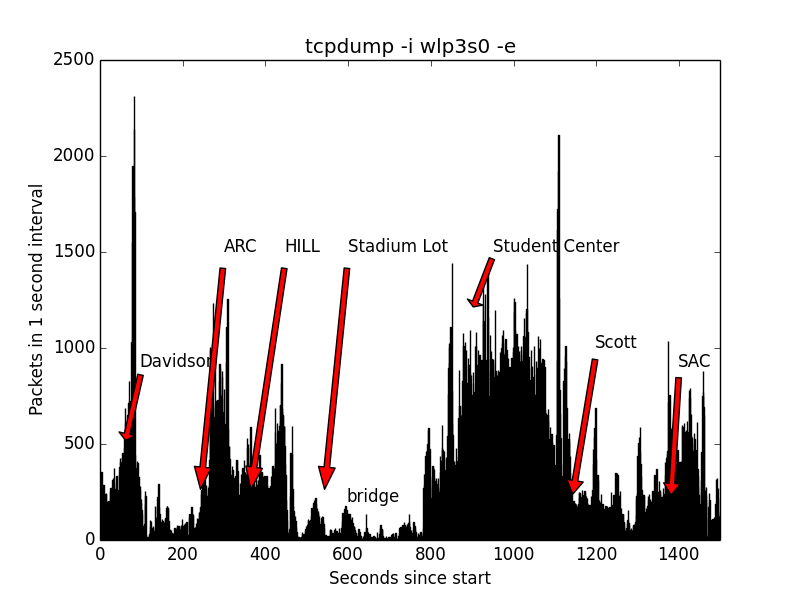
\includegraphics[width=11cm]{packets}
	\\TODO: swap out plot for new data
	\centering
	\end{figure}

	Plotting the number of packets in a histogram with one second bins, we see that there are visible differences between stops.
	There are a few extreme spikes in network traffic, which can be ignored.
	However, this data alone does not establish correlation between traffic and occupancy; since the range of the wireless card extends beyond the bus, there will be considerable noise.
	\\
	tcpdump also records the strength of signals, so we can choose to ignore packets below a certain decibel strength:

	\begin{figure}[H]
	\includegraphics[width=11cm]{strength}
	\\TODO: swap out plot for new data
	\centering
	\end{figure}

	Additionally, we switched out ``number of packets'' for ``number of unique MAC addresses''.

	\begin{figure}[H]
	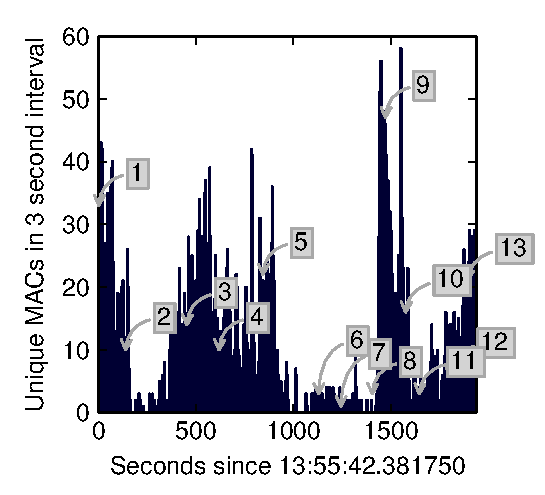
\includegraphics[width=11cm]{unique}
	\\TODO: swap out plot for new data, remake with strength cutoff
	\centering
	\end{figure}

	In order to establish which devices were on the bus, we plotted the time of the first and last occurance of each device:


	\begin{figure}[H]
	\includegraphics[width=11cm]{firstlastbus}
	\centering
	\end{figure}

	Each point here represents a unique device, where the x-coordinate is the time of the first sighting, and the y-coordinate is the time of the last sighting.
	Thus, the high concentration of data points along the line y=x represents the transient devices, most likely all access points.
	The clump of data points at the top left of the plot represents devices which were seen throughout the journey. These are most likely the access points of the common first and last stop.
	\\

	TODO: Conclude


\section*{Future Work}
The largest problem with the interception of packets is outside noise.
To address this, we would like to install an access point on the bus, with the same SSID as the campus Wi-Fi so that smart phones would automatically connect.
We could then listen only to communications with this access point, eliminating outside traffic.
\\
Optimally, the routers would be officially installed and serve mobile data. This is naturally expensive and thus unlikely. Any unofficial access points installed would be an explicit violation of the terms of use of the Rutgers networks, and thus unfeasible as well.
\\
\\
We could also replace the laptop in our setup with a smaller unit to be installed in the busses, to collect data for longer periods of time. Running several of these units would allow us to collect enough data to make occupancy predictions.


\section*{Team Member Contributions}
Here is a list of the contributions made by each individual team member.
\\
\\
Daniel Bordak
\begin{itemize}
  \item Collected bus and classroom data
  \item Annotated grid (first seen, last seen) graphs
  \item Created filter scripts for signal strength and routers
  \item Created script to convert data file into json
\end{itemize}
\vspace{10 mm}
Erin Corrado
\begin{itemize}
  \item Collected bus and classroom data
  \item Created graphs showing the correlations for length of bus stop and occupancy
  \item Created script to generate the grid (first seen, last seen) graphs
  \item Designed and compiled poster
\end{itemize}
\vspace{10 mm}
Revan Sopher
\begin{itemize}
  \item Created script to filter unique MAC addresses from the data
  \item Wrote the abstract and report
  \item Generated histograms showing number of packets and number of unique MAC addresses vs. time
  \item Annotated histogram plots
\end{itemize}
\vspace{10 mm}
Ashley Weaver
\begin{itemize}
  \item Collected bus data
  \item Helped to write and organize text on the poster
\end{itemize}
\end{document}
